%%%%%%%%%%%%%%%%%%%%%%%%%%%%%%%%%%%%%%%%%%%%%%%%%%%%%%%%%%%%%%%%%%%%%%
% LaTeX Example: Project Report
%
% Source: http://www.howtotex.com
%
% Feel free to distribute this example, but please keep the referral
% to howtotex.com
% Date: March 2011 
% 
%%%%%%%%%%%%%%%%%%%%%%%%%%%%%%%%%%%%%%%%%%%%%%%%%%%%%%%%%%%%%%%%%%%%%%
% How to use writeLaTeX: 
%
% You edit the source code here on the left, and the preview on the
% right shows you the result within a few seconds.
%
% Bookmark this page and share the URL with your co-authors. They can
% edit at the same time!
%
% You can upload figures, bibliographies, custom classes and
% styles using the files menu.
%
% If you're new to LaTeX, the wikibook is a great place to start:
% http://en.wikibooks.org/wiki/LaTeX
%
%%%%%%%%%%%%%%%%%%%%%%%%%%%%%%%%%%%%%%%%%%%%%%%%%%%%%%%%%%%%%%%%%%%%%%
% Edit the title below to update the display in My Documents
%\title{Project Report}
%
%%% Preamble
\documentclass[paper=letter, fontsize=10pt]{scrartcl}
\usepackage[T1]{fontenc}
\usepackage{fourier}

\usepackage[english]{babel}															% English language/hyphenation
\usepackage[protrusion=true,expansion=true]{microtype}	
\usepackage{amsmath,amsfonts,amsthm} % Math packages
\usepackage[pdftex]{graphicx}	
\usepackage{url}
\usepackage{enumerate}
\usepackage{lastpage}
\usepackage{float}


%%% Custom sectioning
\usepackage{sectsty}
\allsectionsfont{\normalfont\scshape}


%%% Custom headers/footers (fancyhdr package)
\usepackage{fancyhdr}
\pagestyle{fancy}
\fancyhead[L]{}
\fancyhead[c]{Design Revision 0 Revision 0}
\fancyhead[R]{\today}											
\fancyfoot[L]{}											 
\fancyfoot[C]{}											
\fancyfoot[R]{\thepage\ of \pageref{LastPage}}		% Pagenumbering
\renewcommand{\headrulewidth}{0.4pt}				% Remove header underlines
\renewcommand{\footrulewidth}{0.4pt}				% Remove footer underlines
\setlength{\headheight}{13.6pt}


%%% Equation and float numbering
\numberwithin{equation}{section}		% Equationnumbering: section.eq#
\numberwithin{figure}{section}			% Figurenumbering: section.fig#
\numberwithin{table}{section}				% Tablenumbering: section.tab#


%%% Maketitle metadata
\newcommand{\horrule}[1]{\rule{\linewidth}{#1}} 	% Horizontal rule
\newcommand{\ts}{\textsuperscript}

%%% Begin document
\begin{document}

\begin{titlepage}

\newcommand{\HRule}{\rule{\linewidth}{0.5mm}} % Defines a new command for the horizontal lines, change thickness here
\newcommand{\authors}{\shortstack{Vitaliy Kondratiev,\\Nathan Johrendt,\\Tyler Lyn,\\Mark Gammie}}

\begin{center}
 
%----------------------------------------------------------------------------------------
%	HEADING SECTIONS
%----------------------------------------------------------------------------------------

\textsc{\LARGE McMaster University}\\[1.5cm] % Name of your university/college
\textsc{\Large CAS 4ZP6}\\[0.5cm]
\textsc{\Large Team 9} \\[0.5cm]
\textsc{\Large Capstone Project 2013/2014}\\[0.5cm] % Major heading such as course name
\textsc{\large Porter Simulation}\\[0.5cm] % Minor heading such as course title

%----------------------------------------------------------------------------------------
%	TITLE SECTION
%----------------------------------------------------------------------------------------

\HRule \\[0.4cm]
{ \huge \bfseries Design Revision 0}\\[0.4cm] % Title of your document
\HRule \\[1.5cm]
 
%----------------------------------------------------------------------------------------
%	AUTHOR SECTION
%----------------------------------------------------------------------------------------

\begin{minipage}{0.4\textwidth}
\begin{flushleft} \large
\emph{Authors:}\\
Vitaliy Kondratiev - 0945220\\
Nathan Johrendt - 0950519\\
Tyler Lyn - 0948978\\
Mark Gammie - 0964156\\
\end{flushleft}
\end{minipage}
~
\begin{minipage}{0.4\textwidth}
\begin{flushright} \large
\emph{Supervisor:} \\
Dr. Douglas Down % Supervisor's Name
\end{flushright}
\end{minipage}\\[4cm]

% If you don't want a supervisor, uncomment the two lines below and remove the section above
%\Large \emph{Author:}\\
%John \textsc{Smith}\\[3cm] % Your name

%----------------------------------------------------------------------------------------
%	DATE SECTION
%----------------------------------------------------------------------------------------

{\large \today}\\[3cm] % Date, change the \today to a set date if you want to be precise

%----------------------------------------------------------------------------------------
%	LOGO SECTION
%----------------------------------------------------------------------------------------

%\includegraphics{Logo}\\[1cm] % Include a department/university logo - this will require the graphicx package
 
%----------------------------------------------------------------------------------------
%Template taken from: http://www.softwaretestinghelp.com/test-plan-sample-softwaretesting-and-quality-assurance-templates/

\vfill % Fill the rest of the page with whitespace
\end{center}
\end{titlepage}

\setcounter{tocdepth}{2}

\tableofcontents

\newpage

\section{Revision History}
\begin{center}
    \begin{tabular}{| c | l | l | l |}
    \hline
    Revision \# & Author & Date & Comment \\ \hline
  	1 & \shortstack{\\Vitaliy Kondratiev,\\Nathan Johrendt,\\Tyler Lyn,\\Mark Gammie} & January 11, 2014 & Revision 0 Added to repository \\ \hline
    \end{tabular}
\end{center}

\section{Executive Summary}
\subsection{Introduction}
This document outlines the design decisions, style and methodology for the project of Porter Simulation to be complete for Hamilton Health Sciences.
\subsection{Purpose}
The purpose of this document is to outline the design of each component and how they interface between each other. This document will aid the developers in the development process as well as any future maintenance required.
\subsection{Design Overview}
\section{Implementation Material}
\subsection{Language of Implementation}
Visual Basic in Excel will be used to interface GUI to Simulation Core module. Python Version 2.7.5 will be used for Simulation Core module and all other modules.
\subsection{Supporting Technology and Frameworks}
Simulation will be built on the SimPy 3.0.2 library. GUI will be built in Excel 2010. 
\newpage
\section{Process Diagram}
\begin{figure}[h!]
	\begin{center}
		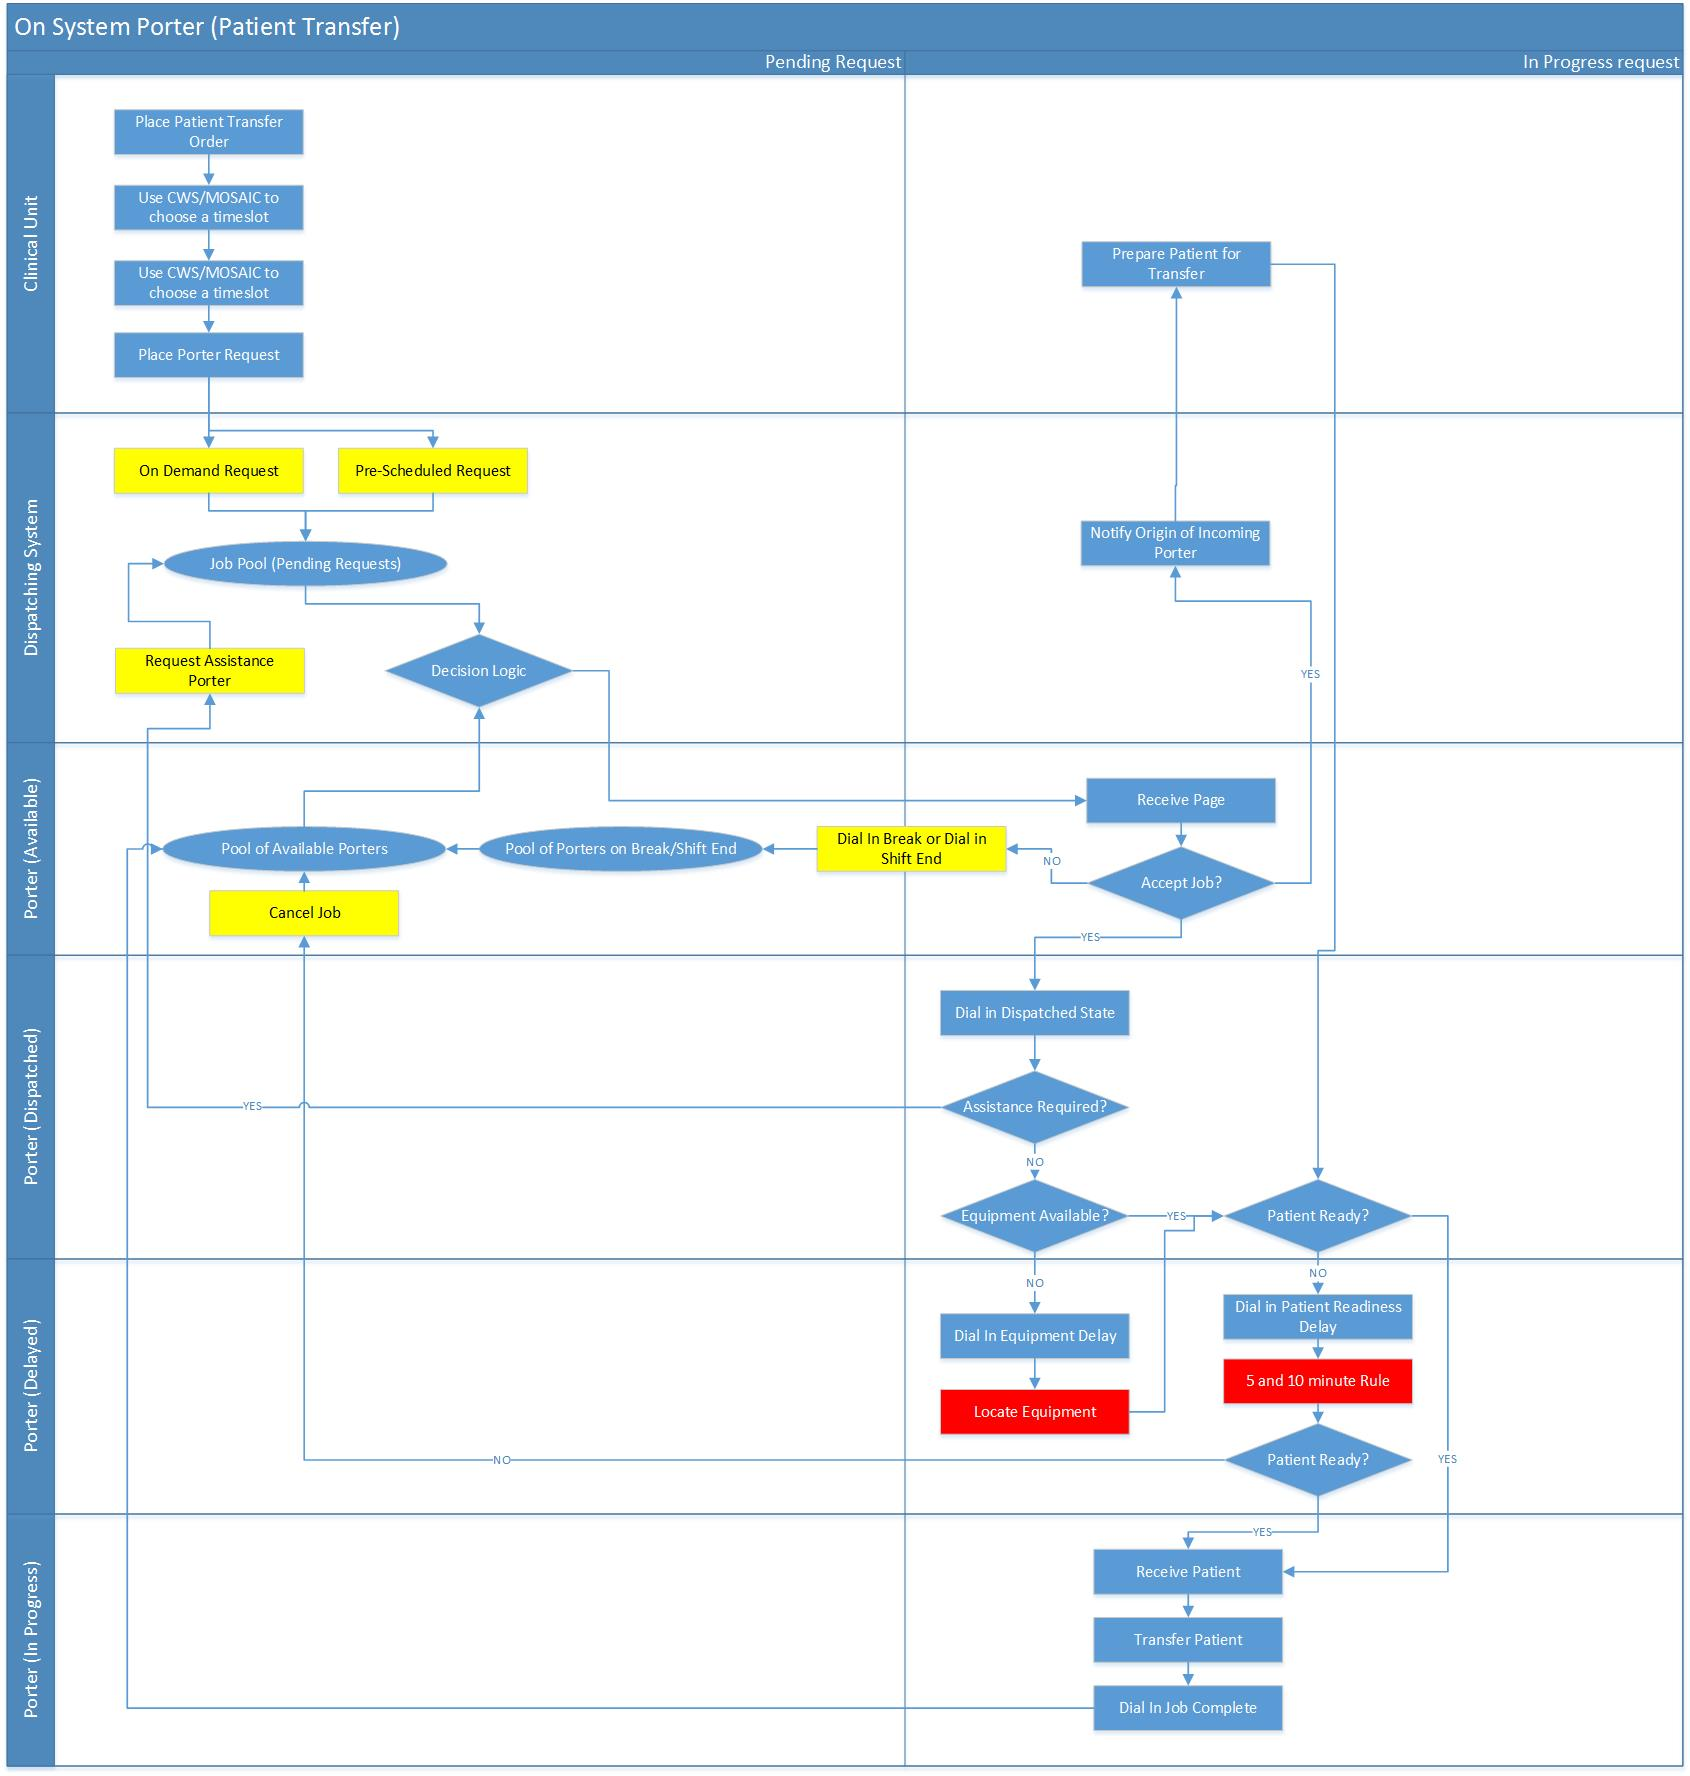
\includegraphics[width=1\columnwidth]{../Process_Diagrams/Process_Diagram.jpg}
		\caption{Process Diagram}
	\end{center}
\end{figure}
\newpage
\section{Dependency Diagram}

\begin{figure}[H]
	\begin{center}
		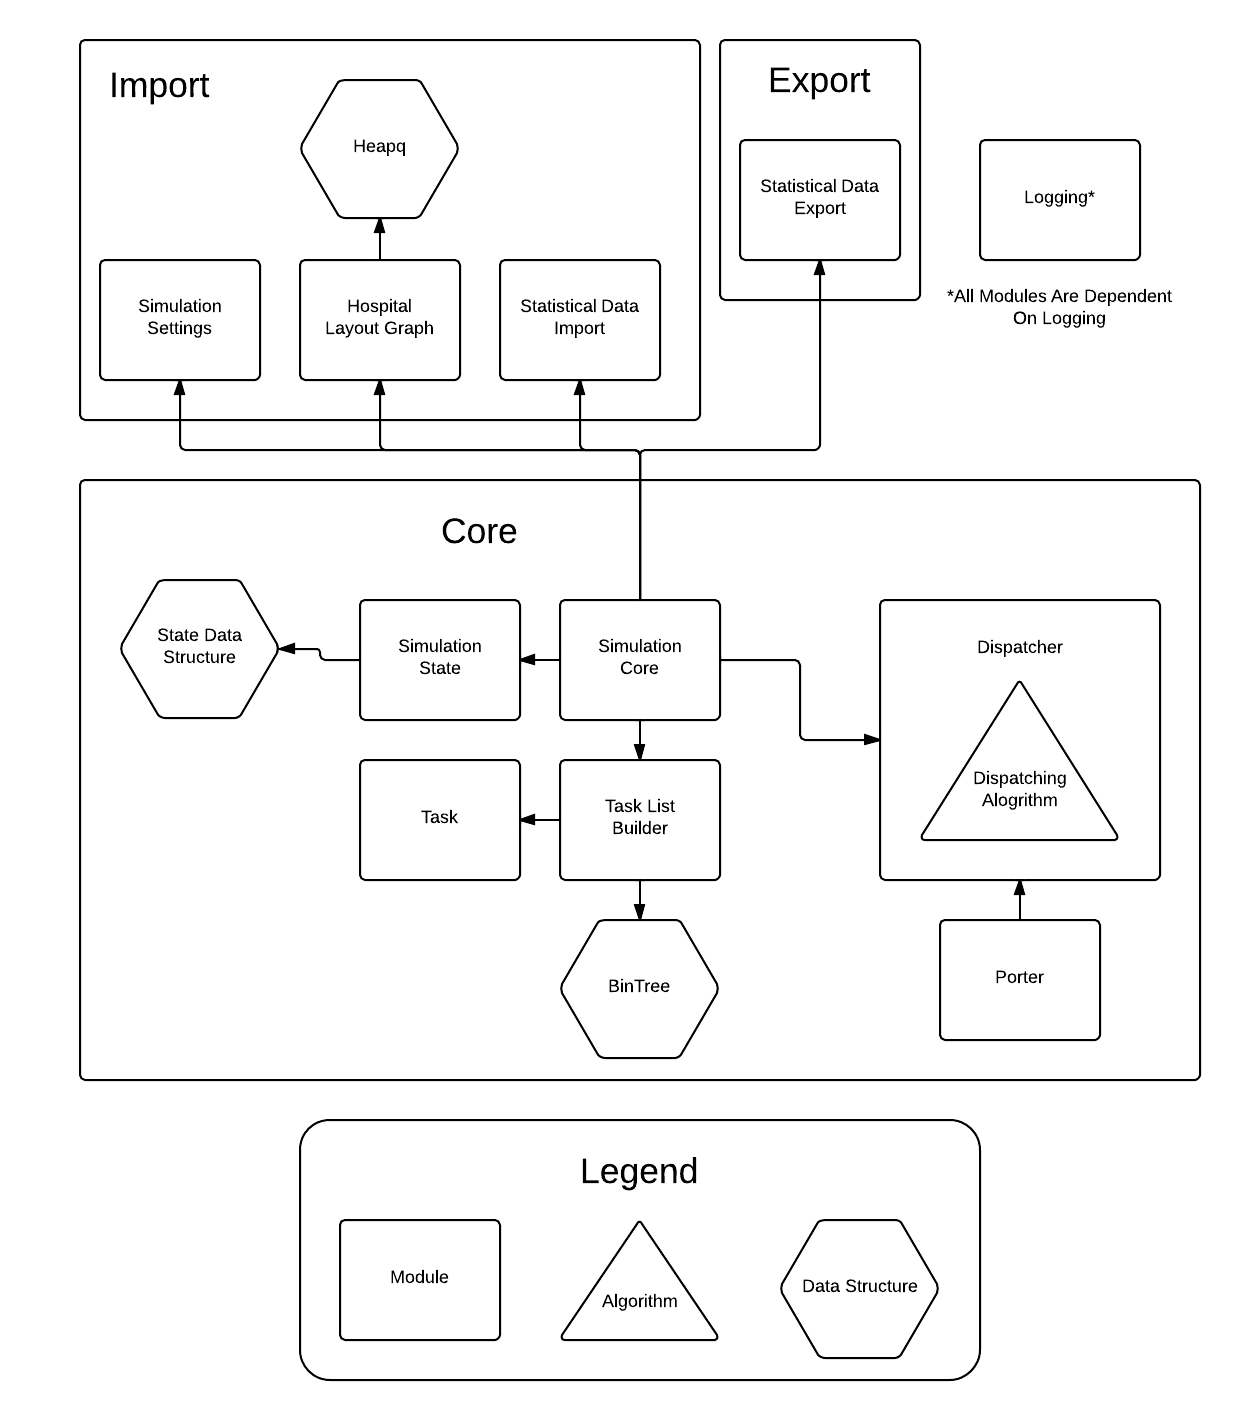
\includegraphics[width=1\columnwidth]{../Process_Diagrams/Dependency_Diagram.png}
		\caption{Dependency Diagram}
	\end{center}
\end{figure}
\newpage

\section{Decomposition Description}
\subsection{Core - Simulation Core}
\begin{enumerate}[]
	\item \textbf{Type:} Module
	\item \textbf{Purpose:} This module calls the required functions to fetch the import data, initializes the simulation and initializes processes.
	\item \textbf{Function:} This module calls the required import modules (Simulation Settings, Hospital Layout Graph, Statistical Data Import), passes their data so that the Simulation State, Event List Builder and Dispatcher can be initialized.
	\item \textbf{Interface:}\\ 
	The interface for the Simulation core is the command line used to called it, defined as follows:
	
	SimCore settings\_filename graph\_filename data\_filename
	
	settings\_filename: the name of the file containing the simulation settings
	
	graph\_filename: the name of the file containing the hospital layout graph
	
	data\_filename: the name of the file containing the statistical data
	
	\item \textbf{Process Steps:} This module first uses the Simulation Settings, Hospital Layout Graph and Statistical data to read in the external data.  This data is used to configure other core modules in the simulation.
	
	Once the external data is imported and the core modules are configured, the Simulation Core will begin the simulation and manage the core modules.
	\item \textbf{Data:} None
	\item \textbf{Error Handling:} Catch all on the simulation loop to report pertinent errors and to prevent unexpected termination. 
	\item \textbf{Requirement Reference:} 11.5
	\item \textbf{Critical Revision 0 Component:} True
\end{enumerate}
\subsection{Core - Simulation State}
\begin{enumerate}[]
	\item \textbf{Type:} Module
	\item \textbf{Purpose:} This module's purpose is to be an interface between the simulation and its simulation state data structure.
	\item \textbf{Function:} This module will contain functions that will be used by the simulation to perform queries on the system state data structure.
	\item \textbf{Interface:}\newline
	initSimulateState():
		\begin{itemize}
			\item Instantiating the simulation state with null values
		\end{itemize}
	getSimulationTime():
		\begin{itemize}
			\item Returns the current simulation time
		\end{itemize}
	getPorterList():
		\begin{itemize}
			\item Returns a list of the porter objects
		\end{itemize}
	
	\item \textbf{Process Steps:} 
	\item \textbf{Data:}
	\item \textbf{Error Handling:}
	\item \textbf{Requirement Reference:}
	\item \textbf{Critical Revision 0 Component:} True
\end{enumerate}
\subsection{Core - Task}
\begin{enumerate}[]
	\item \textbf{Type:} Module
	\item \textbf{Purpose:} 
	\item \textbf{Function:} 
	\item \textbf{Interface:}
	\item \textbf{Process Steps:} 
	\item \textbf{Data:}
	\item \textbf{Error Handling:}
	\item \textbf{Requirement Reference:}
	\item \textbf{Critical Revision 0 Component:} True
\end{enumerate}
\subsection{Core - Event List Builder}
\begin{enumerate}[]
	\item \textbf{Type:} Module
	\item \textbf{Purpose:} Produces the list of events for the Simulation Core module to process
	\item \textbf{Function:} Takes Task List as input to produce Event List
	\item \textbf{Interface:} nextEvent(): upon query takes the top event from the stack and returns it
	\item \textbf{Process Steps:} TBD
	\item \textbf{Data:} Built on BinTree
	\item \textbf{Error Handling:} TBD
	\item \textbf{Requirement Reference:} 8.1 (c)
	\item \textbf{Critical Revision 0 Component:} True
\end{enumerate}
\subsection{Core - Porter}
\begin{enumerate}[]
	\item \textbf{Type:} Module
	\item \textbf{Purpose:}  To complete jobs provided by the dispatcher
	\item \textbf{Function:} Completes the transport jobs assigned by the dispatcher.  Unless a job is cancelled the porter will traverse through four states ('pending', 'dispatched', 'inprogress', 'complete')
	\item \textbf{Interface:} \newline
	setStatePending(state):
		\begin{itemize}
			\item Input the pending state
			\item Sets the porter's state to pending and waits to be assigned a job
		\end{itemize}
	setStateDispatched(state):
		\begin{itemize}
			\item Input the dispatched state
			\item Sets the porter's state to dispatched and calculates the time between the porter's location and the job's origin	
		\end{itemize}
	setStateInprogress(state):
		\begin{itemize}
			\item Input the inprogress state
			\item Sets the porter's state to inprogress and calculates the time between the job's origin and destination.
		\end{itemize}
	setStateComplete(state):
		\begin{itemize}
			\item Input the complete state
			\item Sets the porter's state to complete, records the completion time and sets the porter back to the pending state.
		\end{itemize}
	getAutoLocation():
		\begin{itemize}
			\item Output the estimated location of a pending porter
			\item Estimates the current location of a porter based on how many minutes they have been in the pending state.
		\end{itemize}
	\item \textbf{Process Steps:} The module listens for state changes provided by the dispatcher and updates its' internal components as necessary.
	\item \textbf{Data:} Stores internal data relating to its' current state.
	\item \textbf{Error Handling:} Not Available
	\item \textbf{Requirement Reference:} Not Available
	\item \textbf{Critical Revision 0 Component:} True
\end{enumerate}
\subsection{Core - Dispatcher}
\begin{enumerate}[]
	\item \textbf{Type:} Module
	\item \textbf{Purpose:} To organize pending jobs based on a weighted-value and assign them to porters 
	\item \textbf{Function:} This module orders pending jobs based off of a Dispatch Value which is computed using several parameters (Proximity Match Value, Weighted Job Priority and Appointment Factor).  The pending job with the greatest Dispatch Value will be assigned to the closest available porter.  Once the job is assigned to the porter the job will be considered as a dispatched job.
	\item \textbf{Interface:} \newline
	 assignJob(Job):
	 	\begin{itemize}
	 		\item Assigns the job with the greatest Dispatch Value to the closest available porter.
	 	\end{itemize}
	 getProxmityMatchValue(Job Origin):
	 	\begin{itemize}
	 		\item Input the origin of a pending job
	 		\item Output a value based on how close an available porter is to a job's origin
	 	\end{itemize}
	 getWeightedJobPriority(Job Origin, Job Destination):
	 	\begin{itemize}
	 		\item Input the origin and destination of a pending job
	 		\item Output a value based on the priority of the pending job
	 	\end{itemize}
	 getAppointmentFactor(Job):
	 	\begin{itemize}
	 		\item Input a pending job
	 		\item Update the value for a job depending on if it was pre-scheduled or on-demand.
	 	\end{itemize}
	 getDispatchValue(Job):
	 	\begin{itemize}
	 		\item Input a pending job
	 		\item Compute the DispatchValue for a job: (ProxmityMatchValue + WeightedJobPriority * AppointmentFactor) 
	 	\end{itemize}
	 updateJobPriority(Job):
	 	\begin{itemize}
	 		\item Input a pending job
	 		\item Determine if the pending job has been waiting too long.  If the job has been pending for  a specified amount of time, update it to a higher priority.
	 	\end{itemize}
	\item \textbf{Process Steps:}
	All pending jobs are assessed and given a dispatch value (DV) based on the weighting and values of specified dispatch parameters.
	
	These weights and values are determined using either the location of an available porter or the priority of a pending job.
	
	All of the pending jobs are then ordered from greatest dispatch value to the least.  When there is an available porter the pending job with the greatest dispatch value is given to the closest porter.
	\item \textbf{Data:}
		\begin{itemize}
			\item Pending jobs
		\end{itemize}
	\item \textbf{Error Handling:} Not Available
	\item \textbf{Requirement Reference:} Not Available
	\item \textbf{Critical Revision 0 Component:} True
\end{enumerate}
\subsection{Import - Simulation Setting}
\begin{enumerate}[]
	\item \textbf{Type:} Module
	\item \textbf{Purpose:} 
	\item \textbf{Function:} 
	\item \textbf{Interface:}
	\item \textbf{Process Steps:} 
	\item \textbf{Data:}
	\item \textbf{Error Handling:}
	\item \textbf{Requirement Reference:}
	\item \textbf{Critical Revision 0 Component:} True
\end{enumerate}
\subsection{Import - Hospital Layout Graph}
\begin{enumerate}[]
	\item \textbf{Type:} Module
	\item \textbf{Purpose:} 
	\item \textbf{Function:} 
	\item \textbf{Interface:}
	\item \textbf{Process Steps:} 
	\item \textbf{Data:}
	\item \textbf{Error Handling:}
	\item \textbf{Requirement Reference:}
	\item \textbf{Critical Revision 0 Component:} True
\end{enumerate}
\subsection{Import - Statistical Data Import}
\begin{enumerate}[]
	\item \textbf{Type:} Module
	\item \textbf{Purpose:} 
	\item \textbf{Function:} 
	\item \textbf{Interface:}
	\item \textbf{Process Steps:} 
	\item \textbf{Data:}
	\item \textbf{Error Handling:}
	\item \textbf{Requirement Reference:}
	\item \textbf{Critical Revision 0 Component:} True
\end{enumerate}
\subsection{Export - Statistical Data Export}
\begin{enumerate}[]
	\item \textbf{Type:} Module
	\item \textbf{Purpose:} 
	\item \textbf{Function:} 
	\item \textbf{Interface:}
	\item \textbf{Process Steps:} 
	\item \textbf{Data:}
	\item \textbf{Error Handling:}
	\item \textbf{Requirement Reference:}
	\item \textbf{Critical Revision 0 Component:} True
\end{enumerate}
\subsection{Logging}
\begin{enumerate}[]
	\item \textbf{Type:} Module
	\item \textbf{Purpose:} 
	\item \textbf{Function:} 
	\item \textbf{Interface:}
	\item \textbf{Process Steps:} 
	\item \textbf{Data:}
	\item \textbf{Error Handling:}
	\item \textbf{Requirement Reference:}
	\item \textbf{Critical Revision 0 Component:} True
\end{enumerate}
\subsection{GUI - Basic Settings}
\begin{enumerate}[]
	\item \textbf{Type:} User Interface
	\item \textbf{Purpose:} Allows the user to change the basic setting of the simulation and run the simulation
	\item \textbf{Function:} 
	\begin{enumerate}[]
		\item \textbf{Number of Porters:} specify the number of porters for the simulation to run
		\item \textbf{Start Date:} specify the day the simulation will run from
		\item \textbf{Start Time:} specific time the simulation runs from
		\item \textbf{End Date:} specific time day the simulation will end
		\item \textbf{End Time:} specific time the simulation ends
		\item \textbf{Job Distribution:} users can choose from predefined distributions or base it on existing statistical data
		\item \textbf{Job Intensity:} specify the frequency of job distribution
		\item \textbf{Correct Equipment Usage:} specify the percentage of correct equipment events
		\item \textbf{Patient Readiness:} specify the percentage of ready patients on porter arrival
		\item \textbf{Porter Wait Time:} specify the time a porter waits for patient to be ready before abandoning job		
	\end{enumerate}
	\item \textbf{Interface:}
		\begin{enumerate}[]
			\item \textbf{Advanced Setting:} proceed to Advanced Setting GUI
			\item \textbf{Simulate:} push settings to Simulation Core
			\item \textbf{Default Settings:} reset to default values
		\end{enumerate}
	\item \textbf{Process Steps:} Not Available
	\item \textbf{Data:} Not Available
	\item \textbf{Error Handling:} If any of the below values violates its restriction, excel will not allow the information to be sent to the simulation core.
	\begin{enumerate}[]
		\item \textbf{Number of Porters:} restricts the number of porters to a positive integer 
		\item \textbf{Start Date:} restricts the start date to day/month/year format
		\item \textbf{Start Time:} restricts the start time to 12 or 24 hour time
		\item \textbf{End Date:} restricts the end date to day/month/year format and checks that the date is on the same date or a later date than the start date
		\item \textbf{End Time:} restricts the end time to 12 or 24 hour time and checks that the end time is further in the future than the start time
		\item \textbf{Job Distribution:} user is restricted to a set series of options
		\item \textbf{Job Intensity:} user is restricted to a set series of options
		\item \textbf{Correct Equipment Usage:} restricts the value between 0 and 100 percent 
		\item \textbf{Patient Readiness:} restricts the value between 0 and 100 percent
		\item \textbf{Porter Wait Time:} restricts the value to a minimum of 0		
	\end{enumerate}
	\item \textbf{Requirement Reference:} 10.1.1, 10.1.2, 10.1.3, 10.1.4
	\item \textbf{Critical Revision 0 Component:} True
\end{enumerate}

\newpage
\begin{figure}[H]
	\begin{center}
		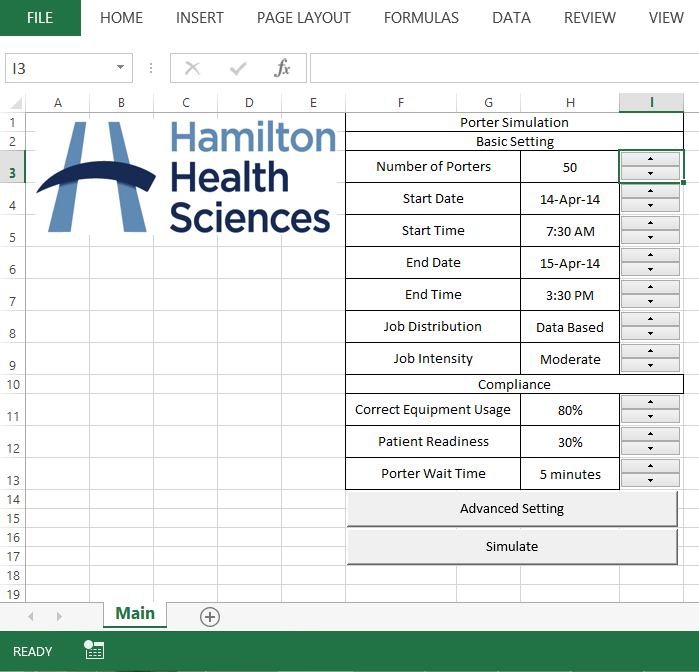
\includegraphics[width=1\columnwidth]{../GUI_Mockups/BasicGUI.png}
		\caption{Basic GUI}
	\end{center}
\end{figure}
\newpage

\section{Anticipated Changes}
\begin{enumerate}[1]
	\item Change 1
\end{enumerate}

%%% End document
\end{document}